\documentclass[compress]{beamer}        % [compress] (written before {beamer} <=> navigation bar one line, all subsections in 1 line instead of 2

% Setup appearance:
\usetheme{CambridgeUS}
%	AnnArbor | Antibes | Bergen |
%	Berkeley | Berlin | Boadilla |
%	boxes | CambridgeUS | Copenhagen |
%	Darmstadt | default | Dresden |
%	Frankfurt | Goettingen |Hannover |
%	Ilmenau | JuanLesPins | Luebeck |
%	Madrid | Malmoe | Marburg |
%	Montpellier | PaloAlto | Pittsburgh |
%	Rochester | Singapore | Szeged |
%	Warsaw
%

\useoutertheme[footline=authorinstitute,subsection=false]{miniframes}
\usecolortheme{whale}

%	albatross | beaver | beetle |
%	crane | default | dolphin |
%	dove | fly | lily | orchid |
%	rose |seagull | seahorse |
%	sidebartab | structure |
%	whale | wolverine


\setbeamertemplate{footline}
{
	\hbox{%
		\begin{beamercolorbox}[wd=.25\paperwidth,ht=2.25ex,dp=1ex,center]{title in head/foot}%
			\usebeamerfont{date in head/foot}\insertshortauthor
		\end{beamercolorbox}%
		\begin{beamercolorbox}[wd=.5\paperwidth,ht=2.25ex,dp=1ex,center]{date in head/foot}%
			\usebeamerfont{title in head/foot}\insertshortinstitute
		\end{beamercolorbox}%
		\begin{beamercolorbox}[wd=.25\paperwidth,ht=2.25ex,dp=1ex,center]{title in head/foot}%
			\usebeamerfont{date in head/foot}
			\insertframenumber{} / \inserttotalframenumber
		\end{beamercolorbox}}%
		\vskip0pt%
	}
	
	%\setbeamercolor{titlelike}{parent=structure}
	%\setbeamercolor{structure}{fg=beamer@blendedblue}
	%% \useinnertheme{rounded}
	%\setbeamerfont{block title}{size={}}
	%\usefonttheme[onlylarge]{structurebold}   % title and words in the table of contents bold
	%\setbeamerfont*{frametitle}{size=\normalsize,series=\bfseries}
	\setbeamertemplate{navigation symbols}{}
	\setbeamercolor{frametitle}{parent=boxes, bg=white}
	
	
	% Standard packages
	\usepackage{graphicx}
	\usepackage[english]{babel}
	\usepackage{framed}
	\usepackage[latin1]{inputenc}
	\usepackage{times}
	\usepackage[T1]{fontenc}
	\usepackage{amsbsy}         % for \boldsymbol command (bold in math mode)
	\usepackage{amsfonts, amssymb}
	\usepackage{epsfig}
	\usepackage{color}
	\definecolor{camblue}{RGB}{26,26,89}
	\definecolor{Rblue}{RGB}{0,255,255}
	\definecolor{Rdarkblue}{RGB}{0,0,255}
	\definecolor{Rgreen}{RGB}{0,205,0}
	\newcommand{\tcb}{\textcolor{beamer@blendedblue}}
	\newcommand{\tcbb}{\textcolor{camblue}}
	\newcommand{\tcr}{\textcolor{red}}
	\newcommand{\tcg}{\textcolor{gray}}
	\newcommand{\tcRg}{\textcolor{Rgreen}}
	\newcommand{\tcRdb}{\textcolor{Rdarkblue}}
	\newcommand{\tcRb}{\textcolor{Rblue}}
	\newcommand{\sq}{\begin{eqnarray}}
	\newcommand{\fq}{\end{eqnarray}}
	\newcommand{\bp}{$\bullet$\:}
	
	
	%%%%%%%%%%%%%%%%%%%%%%%%%%%%%%%%%%%%%%%%%%%%%%%%%%%%%%%%%%%%%%%%%%%%%%%%%%%%%%%%%%%%%%%%%%%%%
	% THIS IS WHERE THE DOCUMENT BEGINS
	
	
	%\setbeamercovered{transparent}   % overlays with light grey 1st slide
	\title
	{
		{\huge Method Comparison Studies \\[0.3cm] }
	}
	\author[Kevin O'Brien]{{\bf Kevin O'Brien (kevin.obrien@ul.ie, University of Limerick)}}
	\institute[University of Limerick, Maths \& Stats Dept]{}
	\date{}
	
	\begin{document}
		
		\begin{frame}
			\vspace{-0.4cm}
%			\begin{center}
%				
\includegraphics[scale = 0.25]{ul_logo.eps}
%			\end{center}
			\titlepage
			
		\end{frame}
		%------------------------------------------------------------------------------%
		
		% Breaking assumptions - using CS and Symmetric VCs
		% LRT implemented using "anova" function
		% JSR Blood data
		
		%------------------------------------------------------------------------------%
		\begin{frame}
			\frametitle{Medical statistics }
			\large
			\begin{figure}
				\centering
				
\includegraphics[width=0.4\linewidth]{images/medstats}
			\end{figure}
			
			\begin{itemize}
				\item Applications to medicine and the health sciences, including epidemiology, public health, forensic medicine, and clinical research. 
				\item "Biostatistics" more commonly connotes all applications of statistics to biology.
				\item Clinical Research is main focus for this talk - Method Comparison Studies
			\end{itemize}
		\end{frame}	
		%================================%
		
		\begin{frame}
			\frametitle{Medical Statistics}
			\large
			\begin{quote} 
				"It is the science of summarizing, collecting, presenting and interpreting data in medical practice, and using them to estimate the magnitude of associations 
				and test hypotheses. 
				
				
				It has a central role in medical investigations. It not only provides a way of organizing information on a wider and more formal basis than relying on the exchange of anecdotes and personal experience, but also takes 
				into account the intrinsic variation inherent in most biological processes." 
				
			\end{quote}
			(Kirkwood, Betty R. (2003). "Essential Medical Statistics")
		\end{frame}
		
		%=================================%
		
		\begin{frame}
			\frametitle{Pharmaceutical statistics}
			\large
			Pharmaceutical statistics is the application of statistics to matters concerning the pharmaceutical industry. \\ \bigskip
			This can be from issues of design of experiments, to analysis of drug trials, to issues of commercialization of a medicine.\\ \bigskip
			There are many professional bodies concerned with this field including:
			\begin{itemize} 
				\item European Federation of Statisticians in the Pharmaceutical Industry (EFSPI)
				\item Statisticians In The Pharmaceutical Industry (PSI)
			\end{itemize}
		\end{frame}
		%================================%
\begin{frame}
	\begin{figure}
\centering

\includegraphics[width=1.1\linewidth]{images/CLSIWebsite}
\end{figure}

\end{frame}		
		%================================%
		\begin{frame}

			\begin{figure}
\centering
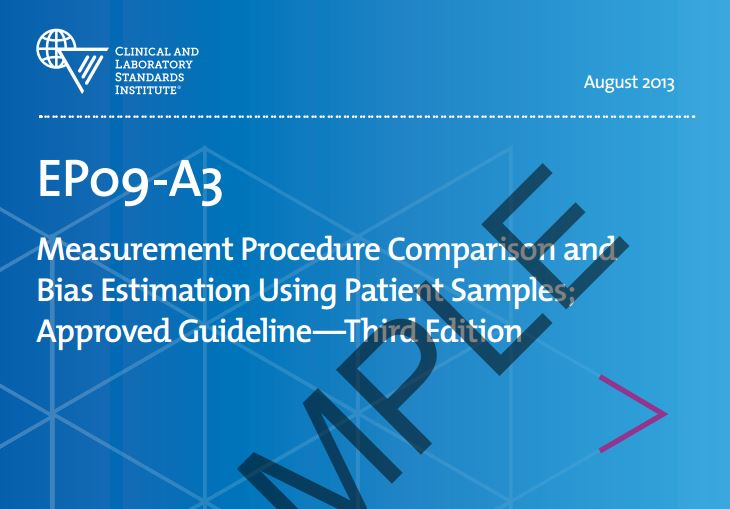
\includegraphics[width=0.9\linewidth]{images/CLSI}

\label{fig:CLSI}
\end{figure}

		\end{frame}
		
		\begin{frame}
			\frametitle{Medical Measurement}
			\begin{figure}
				\centering
				\includegraphics[width=0.4\linewidth]{images/"clinical measurement"}
			\end{figure}
			\begin{figure}
				\centering
				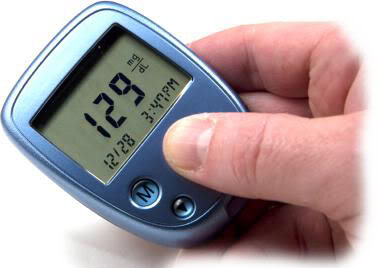
\includegraphics[width=0.35\linewidth]{images/diabetes}
				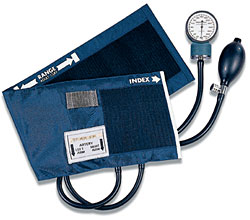
\includegraphics[width=0.35\linewidth]{images/bpcuff}
			\end{figure}
			
		\end{frame}
		%================================================================================ %
		\begin{frame}
			
			\begin{figure}
				\centering
				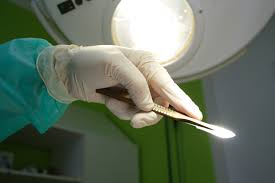
\includegraphics[width=0.7\linewidth]{images/invasiveprocedures}
			\end{figure}
			
		\end{frame}
		
		%------------------------------------------------------------------------%
		\section[Intro to MCS]{Introduction to Method Comparison Studies}
		%\subsection{Method Comparison Studies}
		\begin{frame}{\bf \tcb{Method Comparison Studies}}
			\large
			\begin{itemize}\itemsep0.7cm
				\item Commonly encountered issue in medical statistics
				\item ``Do two methods of measurement agree statistically?".
				\item ``Can the two methods be used interchangeably?"
				\item Sources of disagreement can arise from differing population means (i.e. inter-method bias), differing between-subject and with-in subject variances \cite{Roy2009}.
			\end{itemize}
		\end{frame}
	%======================================================================%
\begin{frame}
\textbf{CRAN Clinical Trials Taskview}	
	\begin{figure}
\centering
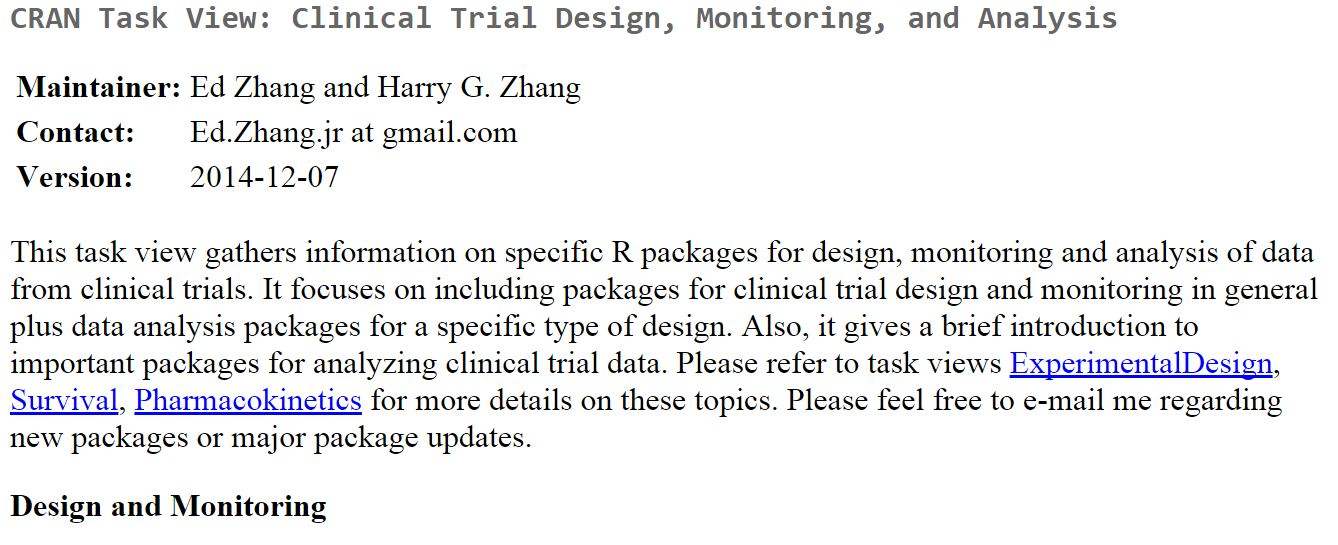
\includegraphics[width=1.1\linewidth]{images/CRAN-clinicaltrials}
\end{figure}

\end{frame}
\begin{frame}
	
	\begin{figure}
		\centering
		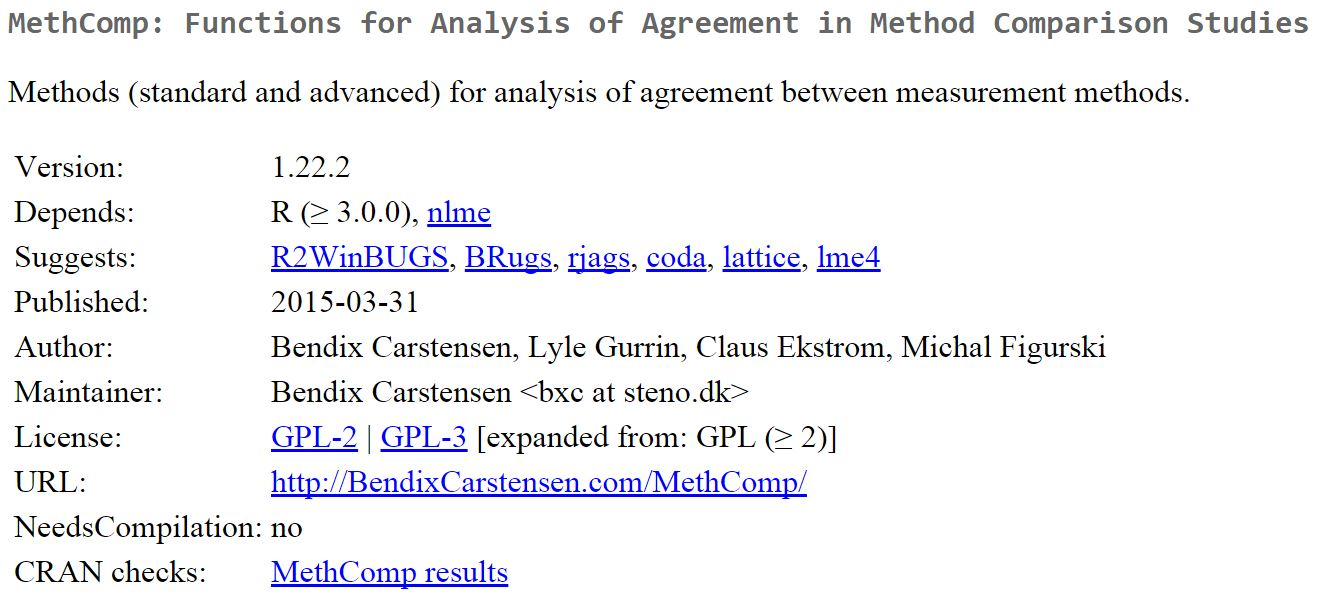
\includegraphics[width=1.05\linewidth]{images/CRAN-MethComp}

	\end{figure}
	
\end{frame}
\begin{frame}
\begin{figure}
\centering
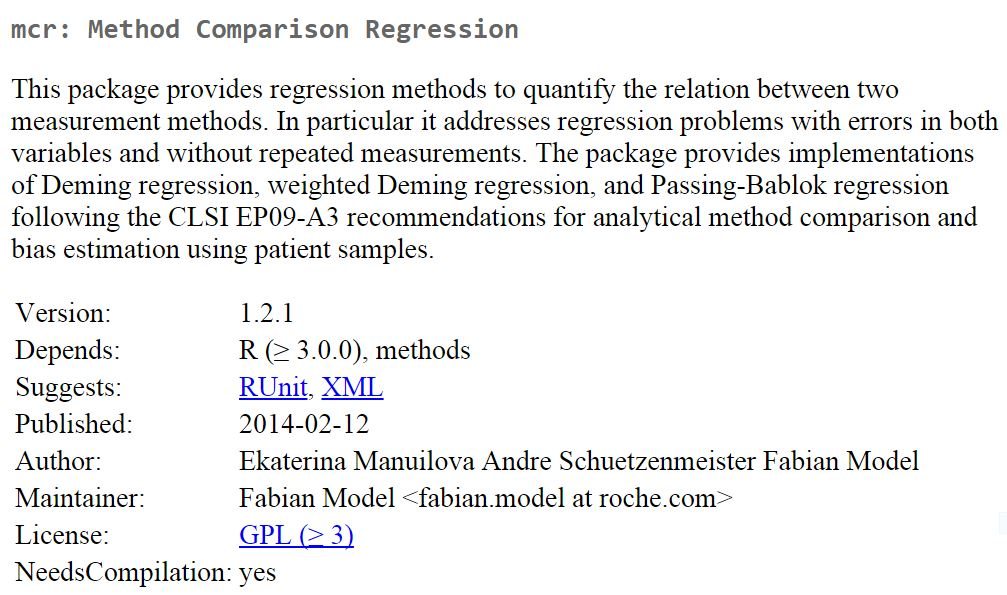
\includegraphics[width=1.05\linewidth]{images/CRAN-mcr}

\end{figure}
\end{frame}

\begin{frame}
	\begin{figure}
\centering
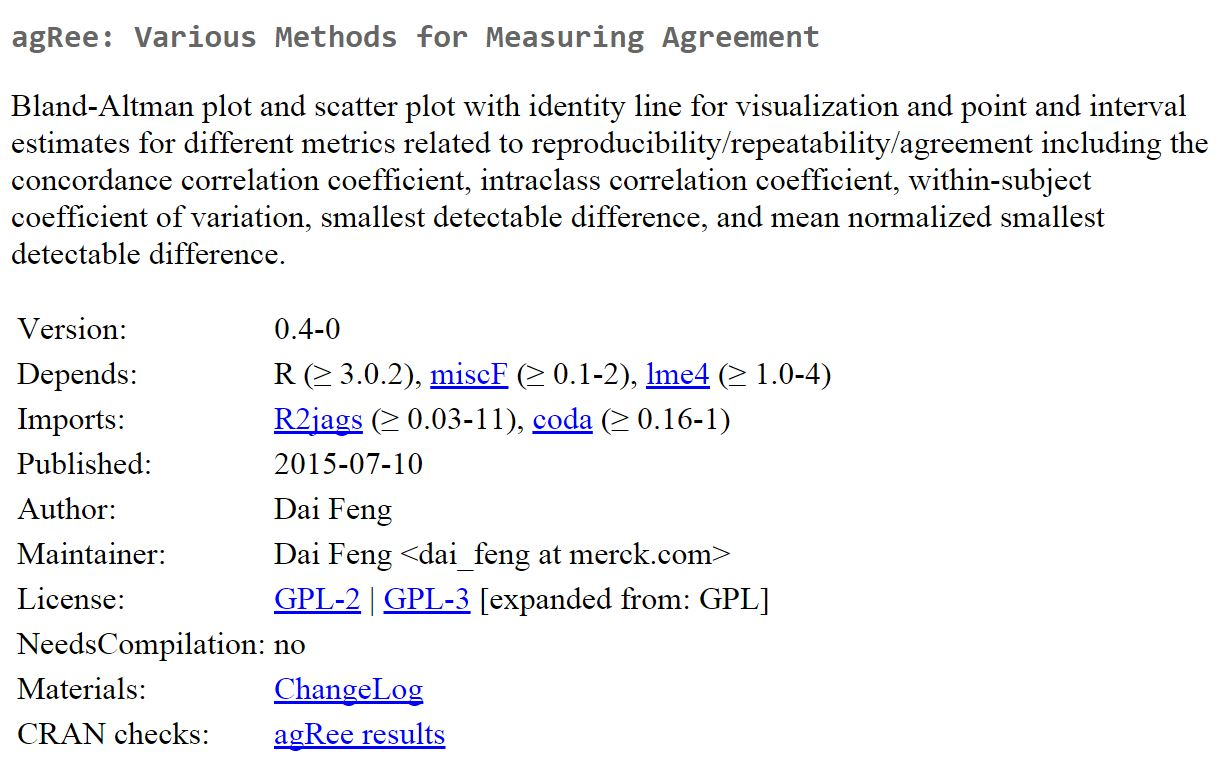
\includegraphics[width=1.05\linewidth]{images/CRAN-agRee}

\end{figure}

\end{frame}
\begin{frame}

	\begin{figure}
\centering
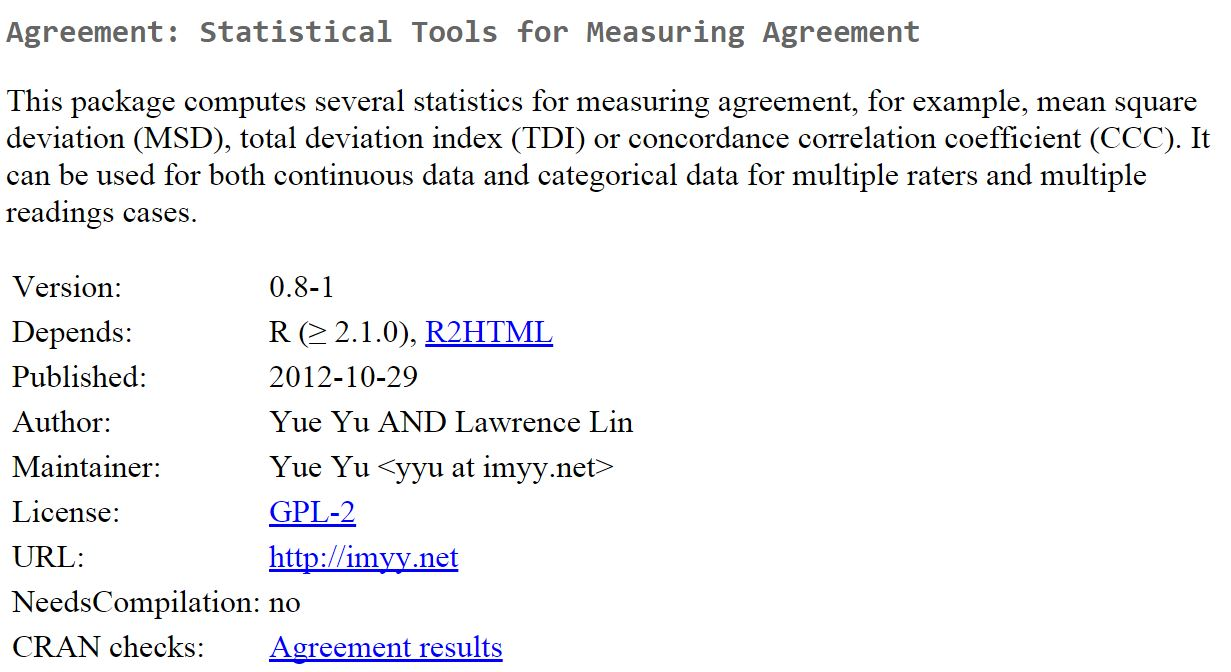
\includegraphics[width=1.05\linewidth]{images/CRAN-agreement}

\end{figure}

\end{frame}	
	%=======================================================================%	
		\begin{frame}
			\frametitle{Gold Standards}
			\large
			\vspace{-1.3cm}
			\textbf{Gold Standard Methods of Measurement}
			\begin{itemize}
				\item	Gold standard test usually refers to a diagnostic test or benchmark that is the best available under reasonable conditions.
				
				
				\item	Other times, gold standard is used to refer to the most accurate test possible without restrictions.
				\item Summary: may yield value close to ``True Value", then again it may not.
			\end{itemize}
		\end{frame}
		
		\begin{frame}
			\large
			\begin{framed}
				\begin{quote}
					For instance, for the diagnosis of aortic dissection, the "gold standard" test used to be the aortogram, which had a sensitivity as low as 83\% and a specificity as low as 87\%. \\ \smallskip
					
					Since the advancements of magnetic resonance imaging, the magnetic resonance angiogram (MRA) has become the new "gold standard" test for aortic dissection, with a sensitivity of 95\% and a specificity of 92\%. 
					\\ \smallskip
					Before widespread acceptance of any new test, the former test retains its status as the "gold standard."
				\end{quote}
			\end{framed}
			
		\end{frame}
		%======================================================================== %
		\begin{frame}
			\frametitle{Methods of Measurement}
			\textbf{Comparing against a Gold Standard}
			\begin{figure}
				\centering
				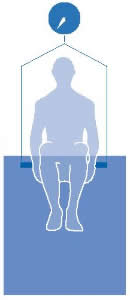
\includegraphics[width=0.18\linewidth]{images/watertest}
				
\includegraphics[width=0.36\linewidth]{images/calipers}
			\end{figure}
			
		\end{frame}
		
		\begin{frame}
			\begin{figure}
				\centering
				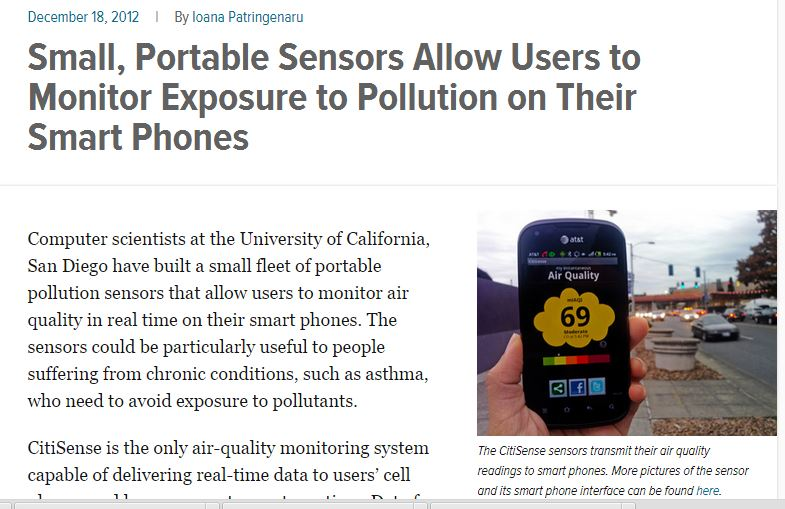
\includegraphics[width=1.05\linewidth]{images/airqualitysensornewsarticle}
				
			\end{figure}
			
		\end{frame}
		%------------------------------------------------------------------------%
		\begin{frame}
			\begin{figure}
\centering
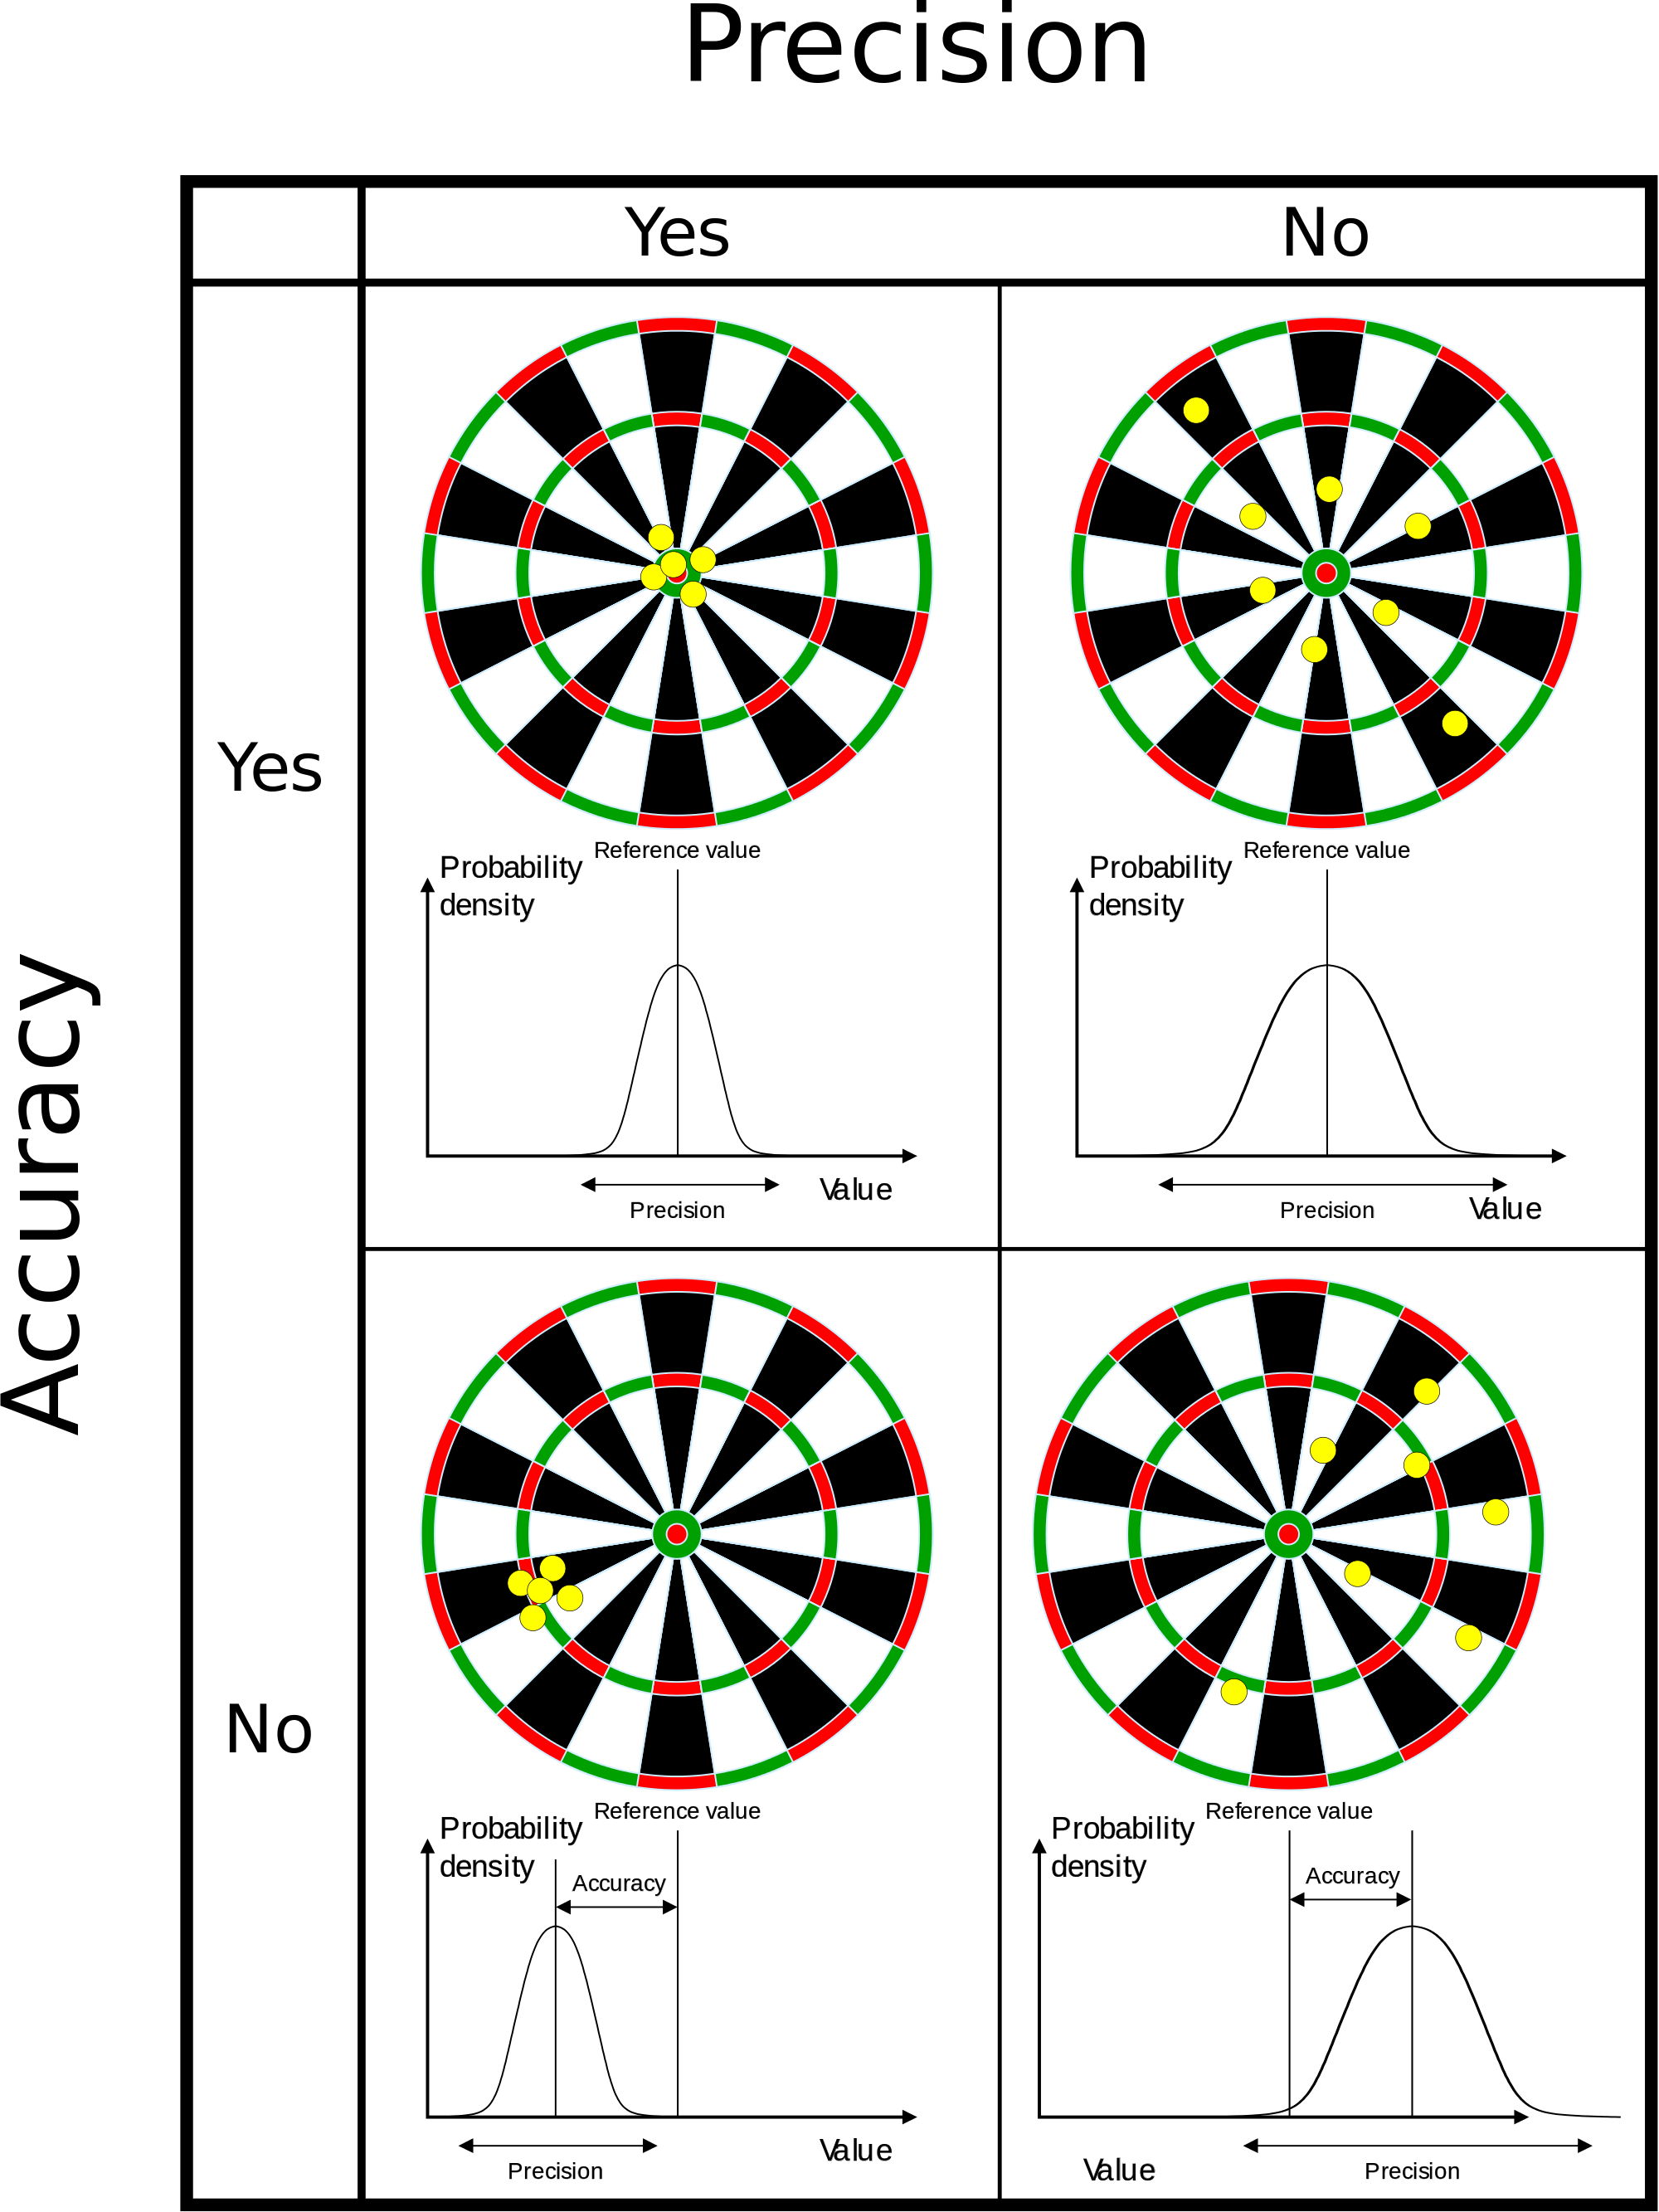
\includegraphics[width=0.45\linewidth]{images/AccuracyPrecision}
\end{figure}
\textit{(Wikipedia.org : Accuracy and Precision.svg)}
		\end{frame}
		\begin{frame}{\bf \tcb{Three Conditions for Agreement}}
			\Large
			For two methods of measurement to be considered interchangeable, the following conditions must apply \cite{Roy2009}:
			\\
			\begin{itemize}\itemsep0.5cm
				\item No significant inter-method bias \textit{(accuracy)}
				\item No difference in the between-subject variabilities of the two methods \textit{(precision)}
				\item No difference in the within-subject variabilities of the two methods \textit{(repeatability)}
			\end{itemize}
		\end{frame}
		%------------------------------------------------------------------------%
		
		\begin{frame}{\bf \tcb{The Bland-Altman Plot}}
			\Large
			\begin{itemize}\itemsep0.7cm
				
				\item The Bland-Altman plot \cite{BA86,BA99} is a very simple graphical method to compare two measurements techniques. \item In this approach the case-wise differences between the two methods are plotted against the corresponding case-wise averages of the two methods.
				
				\item A horizontal lines is drawn at the mean difference(the\textbf{ inter-method bias}) , and at the \textbf{limits of agreement}, which are defined as the inter-method bias plus and minus 2 times the standard deviation of the differences.
				
			\end{itemize}
		\end{frame}
		
		\begin{frame}[fragile]
			\frametitle{Bland-Altman Plot}
			\vspace{-0.3cm}
			\begin{framed}
				\begin{verbatim}
				>X = rnorm(14,6,1);Y = rnorm(14,5.3,1.1)
				>
				>A=(X+Y)/2		#case-wise averages
				>D=X-Y			    #case-wise differences
				>		
				>Dbar=mean(D)	#inter-method bias
				>SdD=sd(D)		#standard deviation of the differences
				>
				>plot(A,D,pch=16,col="red", ylim=c(-3,3))
				>
				>abline(h=Dbar,lty=2)
				>abline(h=(Dbar-2*SdD),lty=2)
				>abline(h=(Dbar+2*SdD),lty=2)
				\end{verbatim}
			\end{framed}
		\end{frame}
		%===================================================================== %
		\begin{frame}
			\vspace{-0.1cm}
			\textbf{Inter-method Bias : 0.27 | Limits of Agreement: [-1.98, 2.52]}
			\vspace{-0.2cm}
			\begin{figure}
				\centering
				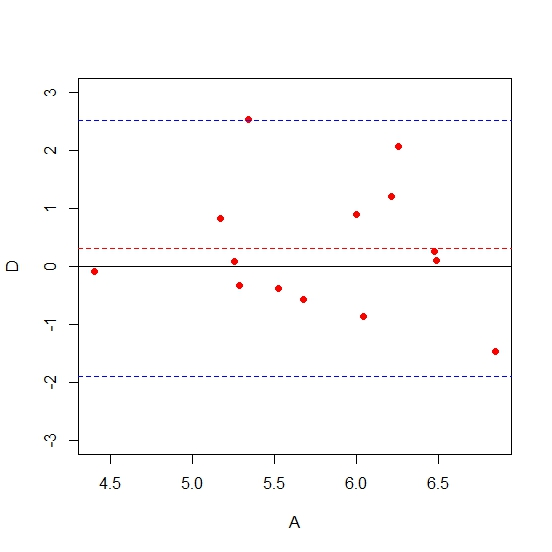
\includegraphics[width=0.7\linewidth]{images/NewBAplot2}
				\label{fig:SimpleBAplot2}
			\end{figure}
			
			
		\end{frame}
		%======================================================================= %
		\begin{frame}[fragile]
			\frametitle{Bland-Altman Plot}
			\vspace{-0.2cm}
			\large
			\textbf{Building Blocks}
			\begin{enumerate}
				\item Simple Arithmetic Operations
				\item Sample Mean  - \texttt{mean()}
				\item Sample Standard deviation - \texttt{sd()}
				\item Scatter plot  - \texttt{plot()}
				\item Normal Distribution 
				\item Enhancing plots  - basic \texttt{R} knowledge 
			\end{enumerate}
			\bigskip
			\textbf{Remark:} Nothing here that is beyond a Stats 101 course in college.
		\end{frame}
		%====================================================================== %
		
		
		
		\begin{frame}
			\textbf{In excess of 32000 citations}
			\begin{figure}
				\centering
				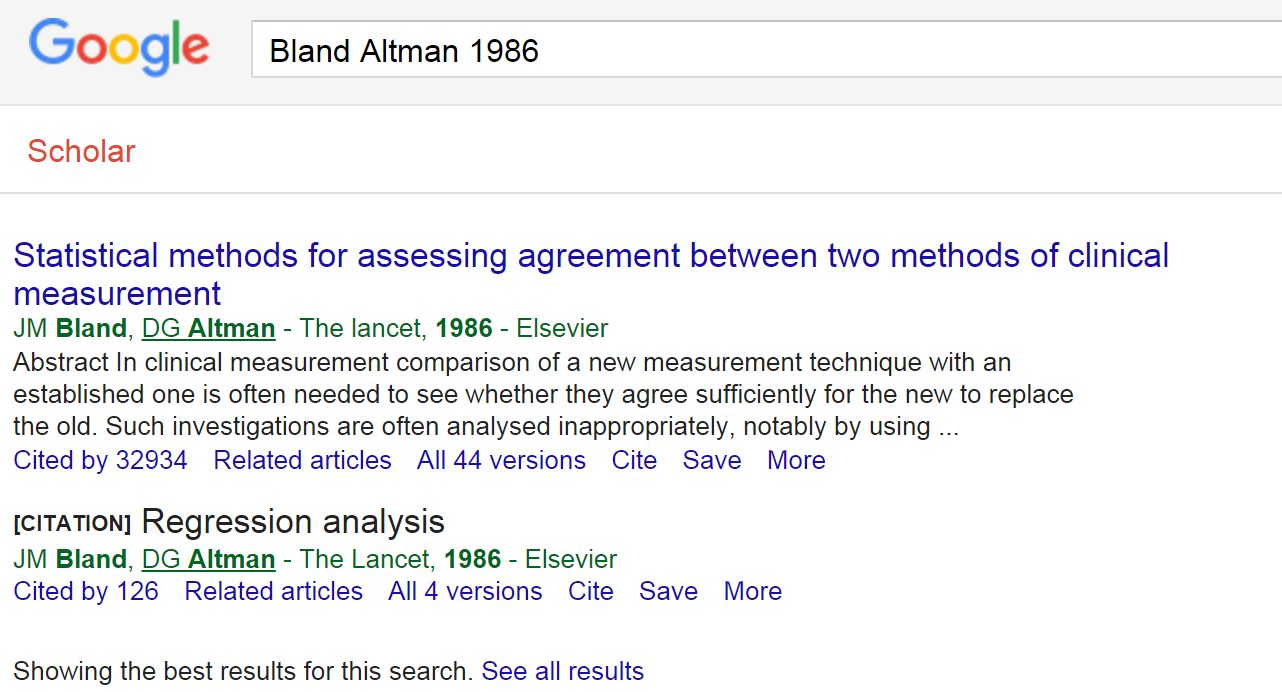
\includegraphics[width=0.9\linewidth]{images/BACITE-dec2015}
				
				\label{fig:BACITE}
			\end{figure}
			
		\end{frame}
				\begin{frame}
					\textbf{May 2015 - In excess of 30000 citations}
					\begin{figure}
						\centering
						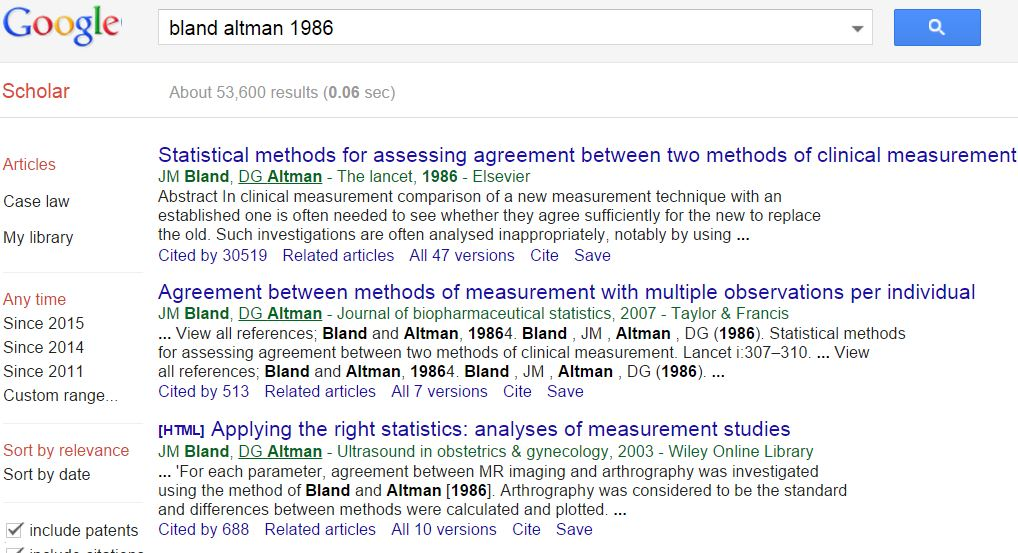
\includegraphics[width=0.9\linewidth]{images/BACITE}
						
						\label{fig:BACITE}
					\end{figure}
					
				\end{frame}
		%======================================================================== %
		\begin{frame}
			\begin{figure}
				\centering
				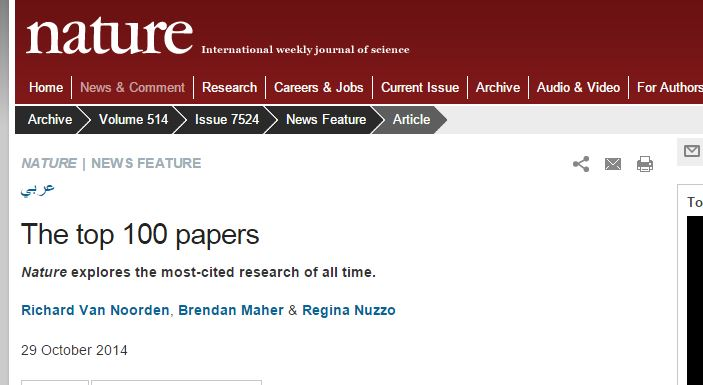
\includegraphics[width=0.99\linewidth]{images/BACITENATURE}
				
				\label{fig:BACITENATURE}
			\end{figure}
			
		\end{frame}
		
		%=================================================================== %
		\begin{frame}
			\begin{figure}
				\centering
				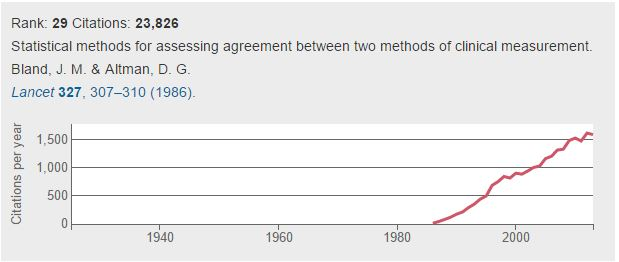
\includegraphics[width=0.99\linewidth]{images/BACITE1}
				
				\label{fig:BACITE1}
			\end{figure}
			
		\end{frame}
		\begin{frame}
			\begin{figure}
\centering
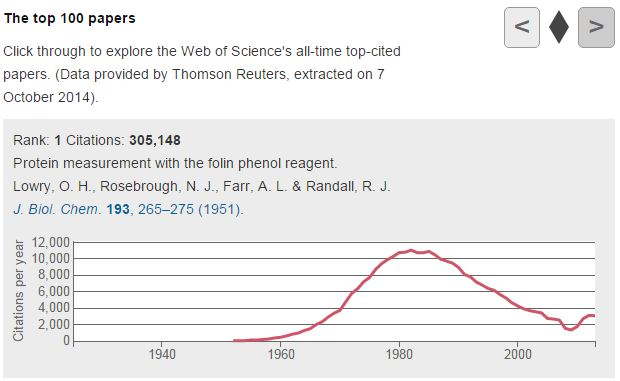
\includegraphics[width=0.99\linewidth]{images/MostCited}

\end{figure}

		\end{frame}
		%==================================================================== %
		\begin{frame}
Nature.com
\begin{framed}
\textit{The Kaplan Meier paper was a sleeper hit, receiving almost no citations until computing power boomed in the 1970s, making the methods accessible to non-specialists. Simplicity and ease of use also boosted the popularity of papers in this field. }\\ \bigskip
	
\textit{British statisticians Martin Bland and Douglas Altman made the list (number 29) with a technique, now known as the Bland Altman plot, for visualizing how well two measurement methods agree. } \\ \bigskip
	
\textit{The same idea had been introduced by another statistician 14 years earlier, but Bland and Altman presented it in an accessible way that has won citations ever since.}
\end{framed}
\textit{(Richard Van Noorden, Brendan Maher\& Regina Nuzzo)	}		
		\end{frame}
		%======================================================================== %
		\begin{frame}
			\frametitle{R Packages for Bland-Altman Analysis}
			\large
			\begin{description}
				\item[PairedData] has a function \texttt{plotBA} based on ggplot2 and no stats as return value
				\item[ResearchMethods] has a function \texttt{BlandAltman} which focuses on a GUI and has no return values.
				\item[epade] has a function \texttt{bland.altman.ade} which appears to have no return values.
				\item[MethComp] has a functino BlandAltman that is deprecated and a function \texttt{ba.plot} which does a lot, mainly regression methods
			\end{description}
		\end{frame}
		%=========================================================================== %

		\begin{frame}
			\frametitle{Interpreting the Bland-Altman Plot}
			
			\begin{figure}
				\centering
				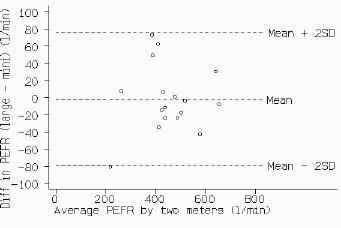
\includegraphics[width=0.95\linewidth]{images/ba2}
				\caption{}
				\label{fig:ba2}
			\end{figure}
			
		\end{frame}
		%======================================================================== %
		\begin{frame}
			\frametitle{Interpreting the Bland-Altman Plot}
			\begin{figure}
				\centering
				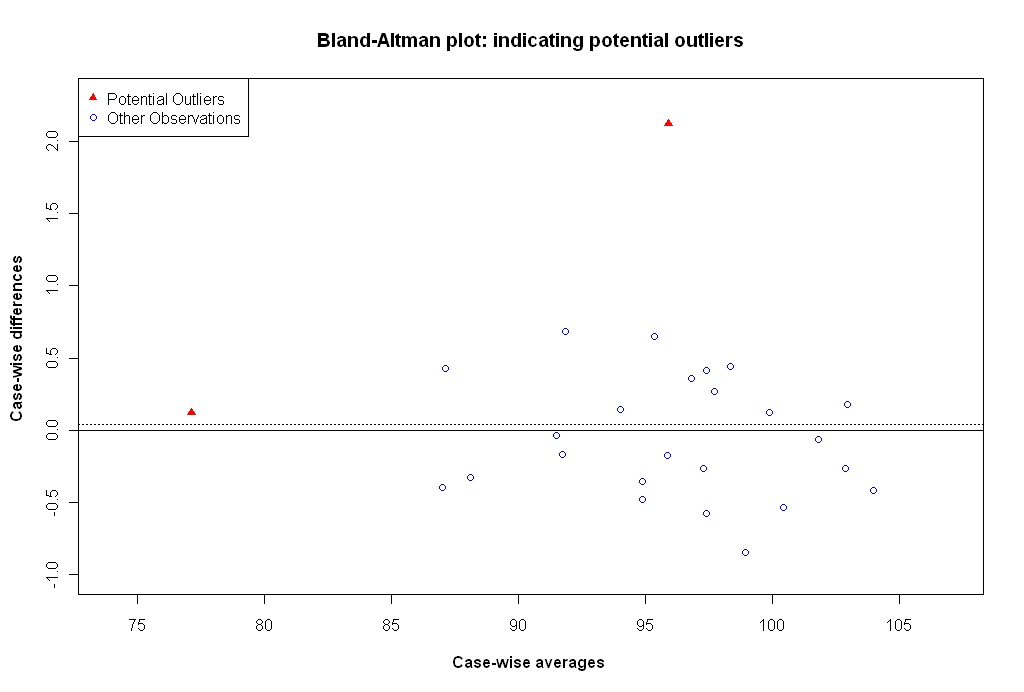
\includegraphics[width=0.85\linewidth]{images/BAOutliers}
				\caption{}
				\label{fig:BAOutliers}
			\end{figure}
			
		\end{frame}
		%======================================================================== %
		\begin{frame}
			\frametitle{Interpreting the Bland-Altman Plot}
			\begin{figure}
				\centering
				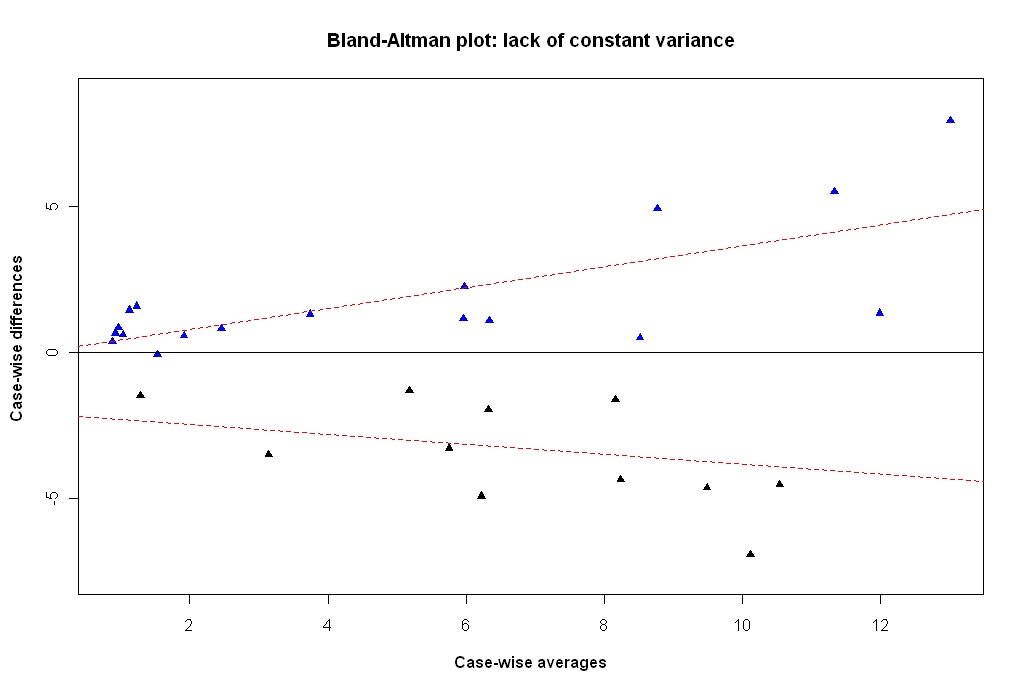
\includegraphics[width=0.85\linewidth]{images/BAFanEffect}
				\caption{}
				\label{fig:BAFanEffect}
			\end{figure}
			
		\end{frame}
		%------------------------------------------------------------------------%
		
		\begin{frame}
			\frametitle{Interpreting the Bland-Altman Plot}
			\begin{figure}
				\centering
				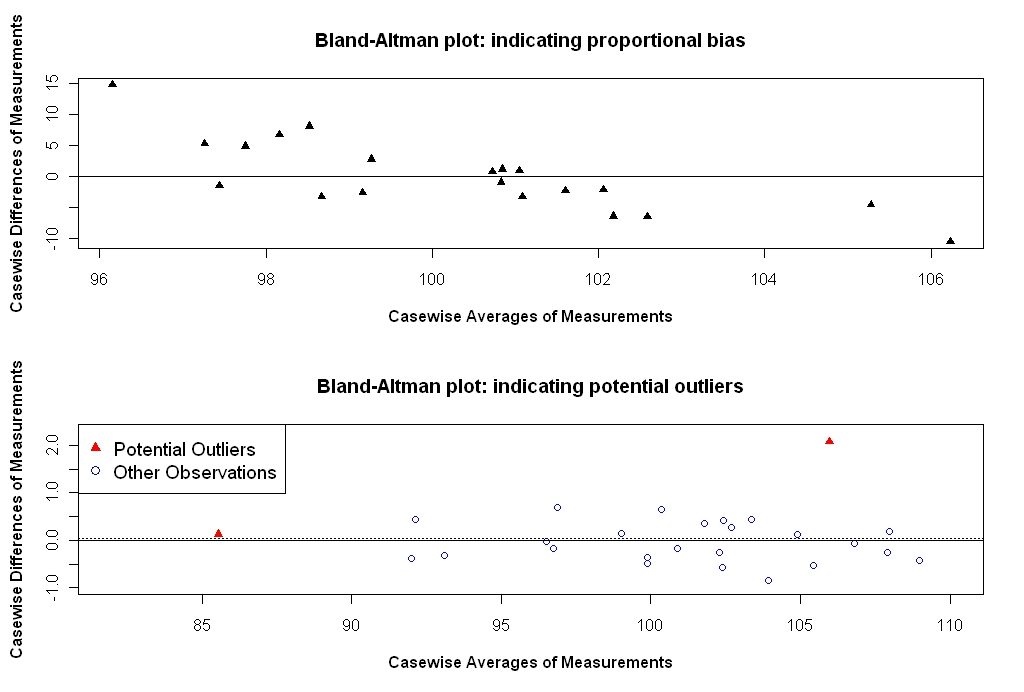
\includegraphics[width=0.9\linewidth]{images/BAcombi}
				\caption{}
				\label{fig:BAcombi}
			\end{figure}
			
		\end{frame}
		%======================================================================== %
		\begin{frame}{\bf \tcb{The Bland-Altman Plot: Prevalence}}
			\large
			\begin{itemize}\itemsep0.7cm
				
				\item Limits of Agreement are used extensively in medical literature for assessing agreement between two methods.
				\item Building Blocks are featured in almost every undergraduate statistics course (i.e. Mean, Standard Deviation, Scatterplot, Normal Distribution)
				\item Other graphical techniques, such as \textit{Survival-Agreement Plot} (based on Kaplan-Meier Curve) and \textit{Mountain Plot} have been developed, but are not prevalent at all.
			\end{itemize}
		\end{frame}
		
		%========================================================================== %
		\begin{frame}
			\frametitle{Survival-Agreement Curve}
\begin{figure}
\centering
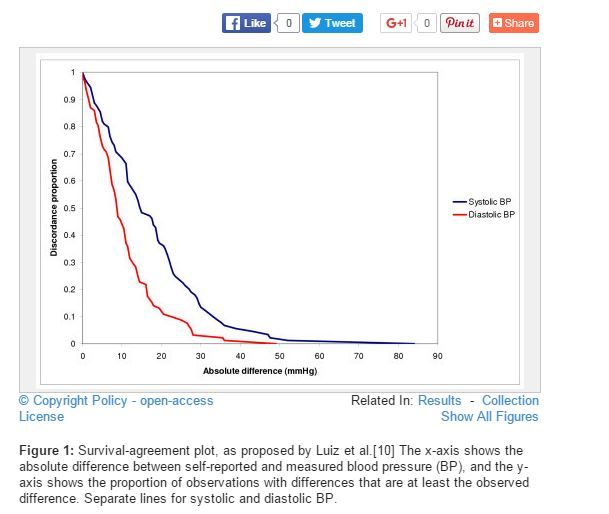
\includegraphics[width=0.7\linewidth]{images/SurvivalAgreementPlot}
\caption{}
\label{fig:SurvivalAgreementPlot}
\end{figure}
			
		\end{frame}
		%========================================================================= %
		\section{TAM and SHINY}
		\begin{frame}
			\frametitle{Technology Acceptance Model}
			\vspace{-0.4cm}
			Davis (1989) proposes the TAM model, which suggests an hypothesis as to why users may adopt particular technologies, and not others. \\ \bigskip
			When users are presented with a new 
			technology, two important factors will influence their decision about how and when they will adopt it.
			\begin{description}
				\item[Perceived usefulness (PU)] - This was defined by Fred Davis as "the degree to which a person believes that using a particular system would enhance his or her job performance".
				\item[Perceived ease-of-use (PEOU)] - Davis defined this as "the degree to which a person believes that using a particular system would be free from effort" 
			\end{description}
		\end{frame}
		%======================================================================= %
		
		\begin{frame}
			\frametitle{Technology Acceptance Model}
			
			\begin{figure}
				\centering
				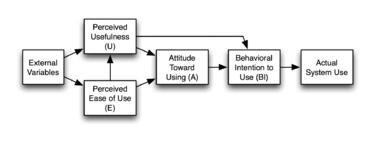
\includegraphics[width=0.89\linewidth]{images/TechAccept}
				\caption{Technology Acceptance Model Flowchart (Davis,1989)}
				\label{fig:TechAccept}
			\end{figure}
			
		\end{frame}
		%====================================================================== %
		
		\begin{frame}
			\Large
			\begin{itemize}
				\item Bland-Altman method not very good on it's own.
				\item Does not account for Replicate Measurements.
				\item Useful as a diagnostic method subsequent to other methods.
				\item Develop a proper methodology for MCS and Get people to use it!
			\end{itemize}
		\end{frame}
		
		%====================================================================== %
		\begin{frame}
			\begin{figure}
				\centering
				
\includegraphics[width=0.99\linewidth]{images/SHINY}
			\end{figure}
			
		\end{frame}
		%==================================================================== %
		
		\begin{frame}
			\frametitle{Shiny Web Applications with R}
			\Large
			\textbf{Useful Shiny Resources}
			\bigskip
			\begin{itemize}
				\item  shiny.rstudio.com \bigskip
				\item  showmeshiny.com \bigskip
				\item  shiny.snap.uaf.edu/ \bigskip
			\end{itemize}
		\end{frame}
		%============================================================================ %
		\begin{frame}
			\begin{figure}
				\centering
				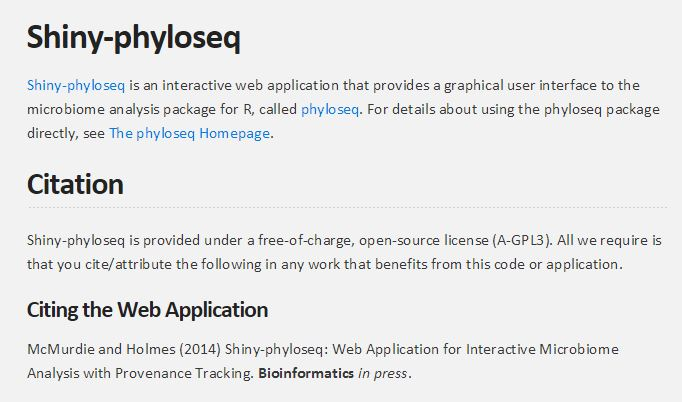
\includegraphics[width=0.99\linewidth]{images/SHINYCITE}
			\end{figure}
			
		\end{frame}
		%------------------------------------------------------------------------%
		
		\begin{frame}{\bf \tcb{Replicate Measurements}}
			\large
			\begin{itemize}\itemsep0.7cm
				\item Bland and Altman's approach originally devised for a single measurement on each item by each of the methods.
				\item Their 1999 paper \cite{BA99} extended their approach to replicate measurements:\\ \emph{By replicates we mean two or more measurements on the same
					individual taken in identical conditions. \\In general this requirement means that the
					measurements are taken in quick succession. }
				\item Emphasis put on "repeatability".
			\end{itemize}
		\end{frame}
		
		%------------------------------------------------------------------------%
		
		\begin{frame}{\bf \tcb{Three Conditions}}
			\Large
			For two methods of measurement to be considered interchangeable, the following conditions must apply \cite{Roy2009}:
			\\
			\begin{itemize}\itemsep0.5cm
				\item No significant inter-method bias
				\item No difference in the between-subject variabilities of the two methods
				\item No difference in the within-subject variabilities of the two methods (repeatability)
			\end{itemize}
		\end{frame}
		
		\section[Roy's LME Model]{Roy's LME Model}
		\subsection{Roy's LME Model}
		%------------------------------------------------------------------------%
		\begin{frame}{\bf \tcb{LME models}}
						\Large
			\begin{itemize}\itemsep0.7cm
				\item In a linear mixed-effects model, responses from a subject are due to both fixed and random
				effects. A random effect is an effect associated with a sampling procedure.
				\item Replicate measurements would require use of random effect terms in model.
				\item Can have differing number of replicate measurements for different subjects.
			\end{itemize}
		\end{frame}
		%------------------------------------------------------------------------%
		\begin{frame}{\bf \tcb{Roy's Approach}}
						\large
			\begin{itemize}\itemsep0.7cm
				\item Roy proposes an LME model with Kronecker product covariance structure in a doubly multivariate setup.
				\item Response for $i$th subject can be written as
				\[ y_i = \beta_0 + \beta_1x_{i1} + \beta_2x_{i2} + b_{1i}z_{i1}  + b_{2i}z_{i2} + \epsilon_i \]
				\item $\beta_1$ and $\beta_2$ are fixed effects corresponding to both methods. ($\beta_0$ is the intercept.)
				\item $b_{1i}$ and $b_{2i}$ are random effects corresponding to both methods.
			\end{itemize}
		\end{frame}
		
		%------------------------------------------------------------------------%
		\begin{frame}{\bf \tcb{Roy's LME model}}
			\large
			\begin{itemize}\itemsep0.7cm
				
				\item Let $\boldsymbol{y}_i$ be the set of responses for subject $i$ ( in matrix form).
				\item $\boldsymbol{y}_i = \boldsymbol{X}_i\boldsymbol{\beta} + \boldsymbol{Z}_i \boldsymbol{b}_i + \boldsymbol{\epsilon}_i$
				\item $\boldsymbol{b}_i \sim N_m(0,\boldsymbol{D})$  (m: number of methods)
				\item $\boldsymbol{\epsilon}_i \sim N_{n_i}(0,\boldsymbol{R})$ ($n_i$: number of measurements on subject $i$)
			\end{itemize}
		\end{frame}
		
		%------------------------------------------------------------------------%
		
		
		\begin{frame}{\bf \tcb{Variance-covariance matrix}}
			\begin{itemize}
				\item Overall variance covariance matrix for response vector $\boldsymbol{y}_i$
				
				\[ \mbox{Var}(\boldsymbol{y}_i)= \boldsymbol{Z}_i \boldsymbol{D}\boldsymbol{Z}^{\prime}_i + \boldsymbol{R}_i \]
				
				\item can be re-expressed as follows:
				\[\boldsymbol{Z}_i \left[ \begin{array}{cc} d^2_1 & d_{12}\\
				d_{12} & d^2_2\\ \end{array}\right]\boldsymbol{Z}^{\prime}_i  +  \left(V \otimes \left[\begin{array}{cc} \sigma^2_1 & \sigma_{12}\\
				\sigma_{12} & \sigma^2_2\\ \end{array}\right] \right)
				\]
				
				\item Overall variability between the two methods is sum of between-subject and within-subject variability,
				\[
				\mbox{Block } \boldsymbol{\Omega}_i = \left[ \begin{array}{cc} d^2_1 & d_{12}\\ d_{12} & d^2_2\\ \end{array} \right]
				+ \left[\begin{array}{cc} \sigma^2_1 & \sigma_{12}\\ \sigma_{12} & \sigma^2_2\\ \end{array}\right].
				\]
				
			\end{itemize}
		\end{frame}
		
		
		
		\section[Implementation]{Implementation}
		\subsection{Implementation}
		
		\begin{frame}{\bf \tcb{Variance-Covariance Structures}}
			\large
			\[\left(
			\begin{array}{cc}
			\sigma^2_1 & \sigma_{12}\\
			\sigma_{12} & \sigma^2_2\\
			\end{array} \right)
			\]
			
			\begin{itemize}
				\item Symmetric structure specifies that $\sigma^2_1$ may differ from $\sigma^2_2$.
				\item Compound symmetric structure specifies that $\sigma^2_1 = \sigma^2_2$.
				\item In both cases, $\sigma_{12}$ may take value other than 0.
			\end{itemize}
			
		\end{frame}
		%------------------------------------------------------------------------%
		\begin{frame}{\bf \tcb{The \texttt{nlme} Package}}
			
			\begin{itemize}
				\item LME models can be implemented in \texttt{R} using the \texttt{nlme} package, one of the core packages.\\
				\item Authors: Jose Pinheiro, Douglas Bates (up to 2007), Saikat
				DebRoy (up to 2002), Deepayan Sarkar (up to 2005), the \texttt{R} Core team \\(source: \texttt{nlme} package manual)\\
				\item ``Mixed-Effects Models in S and S-PLUS" by JC Pinheiro and DM Bates (Springer,2000)
				
			\end{itemize}
			
		\end{frame}
		%-------------------------------------------------------------------%
		\begin{frame}
			\begin{itemize}
				
				\item Recall: Roys uses an LME model approach to provide a set of formal tests for method comparison studies.\\
				
				\item Four candidates models are fitted to the data. One is a reference model, and three are nested models.
				
				\item 
				These models are similar to one another, but for the imposition of equality constraints in the nested models
				
%				\item 
%				The proposed tests are the pairwise comparison of candidate models, one formulated without constraints, the other with a constraint. Constructively tests for equality of variances.\\
				
				
				%Roy's model uses fixed effects $\beta_0 + \beta_1$ and $\beta_0 + \beta_1$ to specify the mean of all observationsby \\ methods 1 and 2 respectively.
			\end{itemize}
		\end{frame}
%-----------------------------------------------------------------------------------%
\begin{frame}
	\frametitle{Variance Covariance Matrices }
	\large
	\begin{itemize}\itemsep0.4cm
		\item Under Roy's model, random effects are defined using a bivariate normal distribution. 
		\item Consequently, the variance-covariance structures can be described using $2 \times 2$  matrices. \item A discussion of the various structures a variance-covariance matrix can be specified under is required before progressing. 
		\item The following structures are relevant:
		\begin{enumerate}
			\item the identity structure, 
			\item the compound symmetric structure
			\item the symmetric structure.
		\end{enumerate}
	\end{itemize}
\end{frame}
%-------------------------------------------%
\begin{frame}
	\frametitle{Variance Covariance Matrices }
	\begin{itemize}
		\item The \textbf{identity} structure is simply an abstraction of the identity matrix. 
		\item The \textbf{compound symmetric} structure and \textbf{symmetric} structure can be described with reference to the following matrix (here in the context of the overall covariance Block-$\boldsymbol{\Omega}_i$, but equally applicable to the component variabilities $\boldsymbol{G}$ and $\boldsymbol{\Sigma}$);
		
		\[\left( \begin{array}{cc}
		\omega^2_1  & \omega_{12} \\
		\omega_{12} & \omega^2_2 \\
		\end{array}\right) \]
	\end{itemize}
\end{frame}

\begin{frame}
	\begin{figure}
\centering
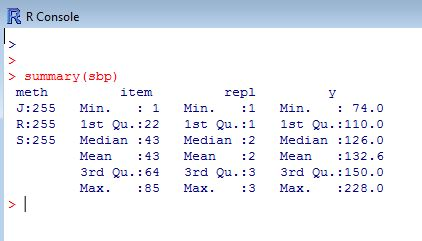
\includegraphics[width=0.9\linewidth]{images/sbpsummary}

\end{figure}

\end{frame}		
\begin{frame}
	\begin{figure}
\centering
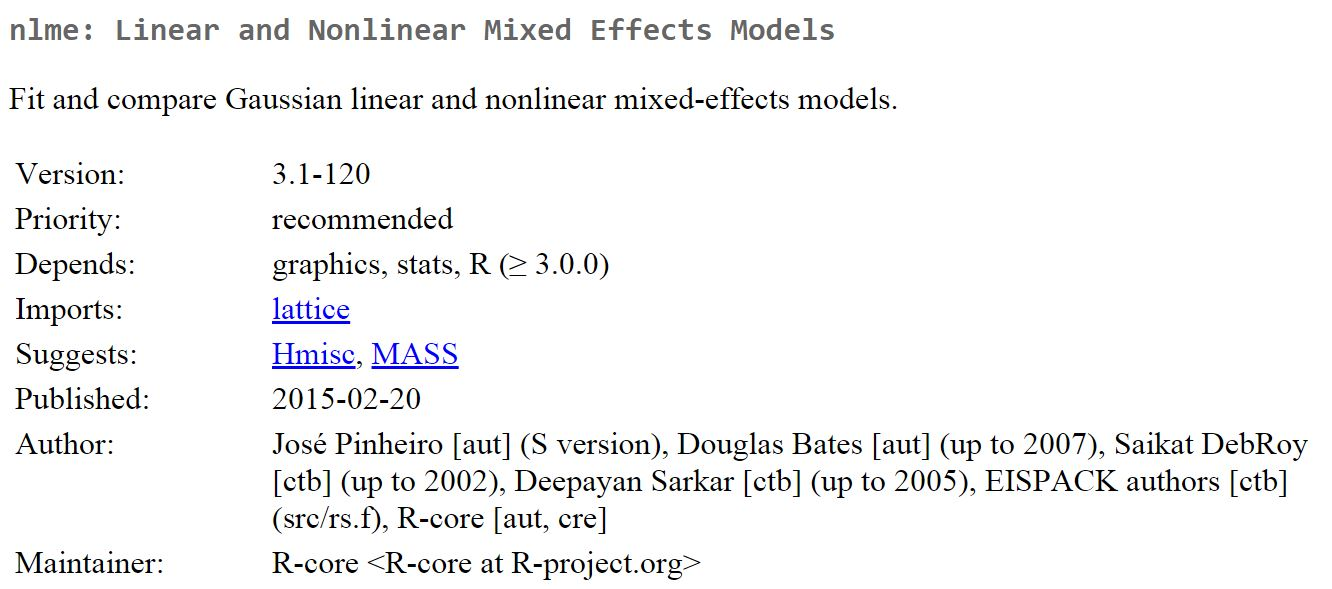
\includegraphics[width=1.1\linewidth]{images/CRAN-nlme}

\end{figure}

\end{frame}
\begin{frame}
	\begin{figure}
\centering

\includegraphics[width=0.6\linewidth]{images/PinheiroBates}

\end{figure}

\end{frame}
		%------------------------------------------------------------------------%
		\begin{frame}[fragile]{\bf \tcb{The Reference Model}}
			\texttt{REF = lme(y $\sim$ meth,\\
				\hspace{0.6cm} data = dat,\\
				\hspace{0.6cm} random = list(item=\tcr{pdSymm}($\sim$ meth-1)), \\
				\hspace{0.6cm} weights=varIdent(form=$\sim$1|meth),\\
				\hspace{0.6cm} correlation = \tcr{corSymm}(form=$\sim$1 | item/repl),\\
				\hspace{0.6cm} method="ML")}\\
			\begin{itemize}
				\item LME model that specifies a symmetric matrix structure for both between-subject and within-subject variances.
			\end{itemize}
			
		\end{frame}
		
		%------------------------------------------------------------------------%
		\begin{frame}[fragile]{\bf \tcb{The Nested Model 1}}
			\texttt{NMB = lme(y $\sim$ meth,\\
				\hspace{0.6cm} data = dat,\\
				\hspace{0.6cm} random = list(item=\tcr{pdCompSymm}($\sim$ meth-1)), \\
				\hspace{0.6cm} weights=varIdent(form=$\sim$1|meth),\\
				\hspace{0.6cm} correlation = \tcr{corSymm}(form=$\sim$1 | item/repl),\\
				\hspace{0.6cm} method="ML")}
			
			\begin{itemize}
				\item LME model that specifies a compound symmetric matrix structure for between-subject and symmetric structure within-subject variances.
			\end{itemize}
			
		\end{frame}
		%------------------------------------------------------------------------%
		\begin{frame}[fragile]{\bf \tcb{The Nested Model 2}}
			\texttt{NMW = lme(y $\sim$ meth,\\
				\hspace{0.6cm} data = dat,\\
				\hspace{0.6cm} random = list(item=\tcr{pdSymm}($\sim$ meth-1)), \\
				\hspace{0.6cm} \tcb{\#weights=varIdent(form=$\sim$1|meth),}\\
				\hspace{0.6cm} correlation = \tcr{corCompSymm}(form=$\sim$1 | item/repl),\\
				\hspace{0.6cm} method="ML")}
			\begin{itemize}
				\item LME model that specifies a symmetric matrix structure for between-subject and compound symmetric structure within-subject variances.
			\end{itemize}
		\end{frame}
		%------------------------------------------------------------------------%
		
		\begin{frame}[fragile]{\bf \tcb{The Nested Model 3}}
			\texttt{NMO = lme(y $\sim$ meth,\\
				\hspace{0.6cm} data = dat,\\
				\hspace{0.6cm} random = list(item=\tcr{pdCompSymm}($\sim$ meth-1)), \\
				\hspace{0.6cm} \tcb{\#weights=varIdent(form=$\sim$1|meth),}\\
				\hspace{0.6cm} correlation = \tcr{corCompSymm}(form=$\sim$1 | /repl),\\
				\hspace{0.6cm} method="ML")}
			\begin{itemize}
				\item LME model that specifies a compound symmetric matrix structure for both between-subject and within-subject variances.
			\end{itemize}
		\end{frame}
		
		
		
		%------------------------------------------------------------------------%
		\section[Example]{Example}
		\subsection{Example}
		\begin{frame}{\bf \tcb{Example: Blood Data}}
			\begin{itemize}\itemsep0.7cm
				\item Used in Bland and Altman's 1999 paper \cite{BA99}. Data was supplied by Dr E O'Brien.
				\item Simultaneous measurements of systolic blood pressure each made by two experienced observers, J and R, using a  sphygmometer.
				\item Measurements also made by a semi-automatic blood pressure monitor, denoted S.
				\item On 85 patients, 3 measurement made in quick succession by each of the three observers (765 measurements in total)
			\end{itemize}
		\end{frame}
		%------------------------------------------------------------------------%
		
		\begin{frame}[fragile]{\bf \tcb{Example: Blood Data}}
			Inter-method Bias between J and S:         15.62 mmHg
			\begin{verbatim}
			>summary(REF)
			.....
			Fixed effects: y ~ meth
			Value Std.Error  DF t-value p-value
			(Intercept) 127.41    3.3257 424  38.310       0
			methS        15.62    2.0456 424   7.636       0
			.....
			\end{verbatim}
		\end{frame}
		%------------------------------------------------------------------------%
		
		\begin{frame}[fragile]{\bf \tcb{Between-subject variance covariance matrix }}
			
			\begin{verbatim}
			..
			Random effects:
			Formula: ~method - 1 | subject
			Structure: General positive-definite
			StdDev    Corr
			methodJ  30.396975 methdJ
			methodS  31.165565 0.829
			Residual  6.116251
			..
			\end{verbatim}
			\[
			\hat{\boldsymbol{D}} = \left(
			\begin{array}{cc}
			923.97	& 785.34 \\
			785.34	& 971.29\\
			\end{array}\right)
			\]
		\end{frame}
		
		%------------------------------------------------------------------------%
		\begin{frame}[fragile]{\bf \tcb{Within-subject variance covariance matrix}}
			\begin{verbatim}
			Correlation Structure: General
			Formula: ~1 | subject/obs
			Parameter estimate(s):
			Correlation:
			1
			2 0.288
			Variance function:
			Structure: Different standard deviations per stratum
			Formula: ~1 | method
			Parameter estimates:
			J        S
			1.000000 1.490806
			\end{verbatim}
			\[
			\hat{\boldsymbol{\Sigma}} = \left(
			\begin{array}{cc}
			37.40 & 16.06 \\
			16.06 & 83.14 \\
			\end{array}\right)
			\]
		\end{frame}
		%------------------------------------------------------------------------%
		\begin{frame}[fragile]{\bf \tcb{Overall variance covariance matrix}}
			
			\begin{itemize}\itemsep0.7cm
				\item Overall variance \[
				\mbox{Block }\hat{\boldsymbol{\Omega}} = \hat{\boldsymbol{D}} + \hat{\boldsymbol{\Sigma}} =
				\left(
				\begin{array}{cc}
				961.38 & 801.40 \\
				801.40 & 1054.43 \\
				\end{array}
				\right)
				\]
				
				\item Standard deviation of the differences can be computed accordingly : 20.32 mmHg.
				
				\item Furthermore, limits of agreement can be computed: $[15.62 \pm (2 \times 20.32) ]$ (mmHg).
			\end{itemize}
		\end{frame}
		
		%------------------------------------------------------------------------%
		
		\begin{frame}{\bf \tcb{Some useful \texttt{R} commands}}
			\begin{itemize}
				
				\item \texttt{intervals} :\vspace{0.25cm} \\This command obtains the estimate and confidence intervals on the parameters associated with the model.\\
				This is particularly useful in writing some code to extract estimates for inter-method bias and variances, and hence estimates for the limits of agreement.
				
				\item \texttt{anova} : \vspace{0.25cm} \\When a reference model and nested model are specified as arguments, this command performs a likelihood ratio test.
			\end{itemize}
		\end{frame}
		
		
		%------------------------------------------------------------------------%
		\begin{frame}[fragile]{\bf \tcb{Formal Tests: Between-subject Variances}}
			\begin{itemize}
				\item Test the hypothesis that both methods have equal between-subject variances.
				\item Constructed an alternative model ``Nested Model B" using \textbf{\emph{compound symmetric}} form for between-subject variance (hence specifying equality of between-subject variances).
				\item Use a likelihood ratio test to compare models.
			\end{itemize}
			\begin{verbatim}
			...
			> anova(REF,NMB)
			Model df ...     logLik   Test   L.Ratio p-value
			REF    1  8 ...  -2030.736
			NMB    2  7 ...  -2030.812 1 vs 2 0.1529142  0.6958
			...
			\end{verbatim}
			\begin{itemize}
				\item Fail to reject hypothesis of equality.
			\end{itemize}
		\end{frame}
		
		%------------------------------------------------------------------------%
		\begin{frame}[fragile]{\bf \tcb{Formal Tests: Within-subject Variances}}
			\begin{itemize}
				\item Test the hypothesis that both methods have equal within-subject variances.
				\item Constructed an alternative model ``Nested Model W" using compound symmetric form for within-subject variance (hence specifying equality of within-subject variances).
				\item Again, use a likelihood ratio test to compare models.
			\end{itemize}
			\begin{verbatim}
			...
			> anova(REF,NMW)
			Model df ...    logLik   Test  L.Ratio p-value
			REF     1  8 ... -2030.736
			NMW     2  7 ... -2045.044 1 vs 2 28.61679  <.0001
			\end{verbatim}
			\begin{itemize}
				\item Reject hypothesis of equality.
			\end{itemize}
		\end{frame}
		%------------------------------------------------------------------------%
		\begin{frame}[fragile]{\bf \tcb{Formal Tests : Outcomes}}
			\begin{itemize}
				\item Inter-method bias: Significant difference in mean values detected.\\
				\vspace{0.25cm}\item Between-subject variance: No significant difference in between-subject variances between the two methods detected.\\
				\vspace{0.25cm}\item Within-subject variance: A significant difference in within-subject variances is detected.\\
				\vspace{0.25cm}\item Can not recommend switching between the two methods.
			\end{itemize}
		\end{frame}
		%------------------------------------------------------------------------%
		\begin{frame}[fragile]{\bf \tcb{Remarks}}
			\begin{itemize}
				\item Can perform a test for equality of overall variances.\\
				\vspace{0.25cm}\item This can be done by specifying a compound symmetry structure for both between-subject and within-subject variances when constructing a nested model.\\
				\vspace{0.25cm}\item Roy controls the family-wise error rate in paper, using Bonferroni correction procedure.
			\end{itemize}
		\end{frame}
		%------------------------------------------------------------------------%
		\section[References]{References}
		\subsection{References}
		\begin{frame}{\bf \tcb{References}}
			\begin{thebibliography}{99}
				\bibitem{Roy2009} A Roy (2009): \emph{An application of linear mixed effects model to assess the agreement between two methods with replicated observations} Journal of Biopharmaceutical Statistics
				\bibitem{BA86} Bland JM, Altman DG (1986) \emph{Statistical method for assessing agreement between two methods of clinical measurement}.
				\bibitem{BA99} Bland JM, Altman DG (1999)  \emph{Measuring agreement in method comparison studies.} Statistical Methods in Medical Research
				\bibitem{PB} Pinheiro JC, Bates DM (2000): \emph{Mixed-effects models in S and S-PLUS},
				Springer.
				%\bibitem{BXC2008} B Carstensen, J Simpson, and LC Gurrin (2008): \emph{ Statistical models for assessing agreement in method comparison studies with replicate measurements.} International Journal of Biostatistics.
			\end{thebibliography}
		\end{frame}
		
		%------------------------------------------------------------------------%
		
		\begin{frame}{\bf \tcb{Thanks}}
			\begin{itemize}
				\item Dr Kevin Hayes, University of Limerick
				\item Dr Kevin Burke, University of Limerick
				\item Peter Fennell
			\end{itemize}
		\end{frame}
		
		
	\end{document} 